\FloatBarrier

\begin{figure}[h!]
	\centering
	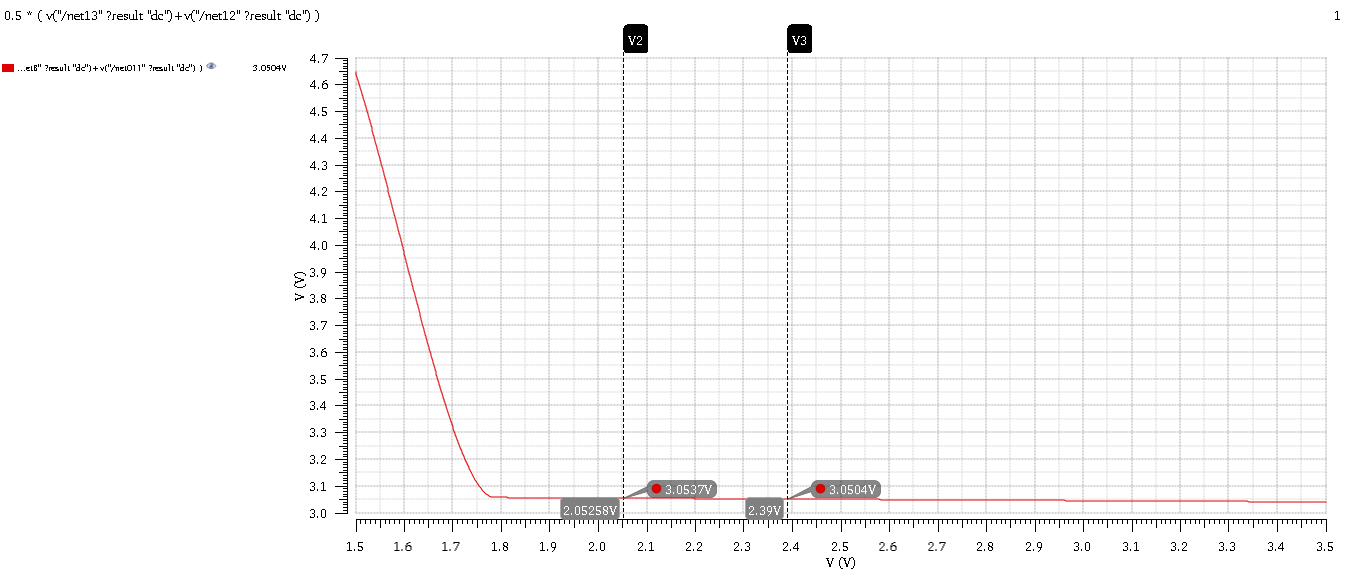
\includegraphics[scale=0.40]{./images/sim3.PNG}
	\caption{$V_{out,cm}$ versus $V_{in,cm}$}
	\label{fig:sim3}
\end{figure}

\FloatBarrier

In order to determine where saturation begins or ends, a wider DC sweep must be taken.

\FloatBarrier

\begin{figure}[h!]
	\centering
	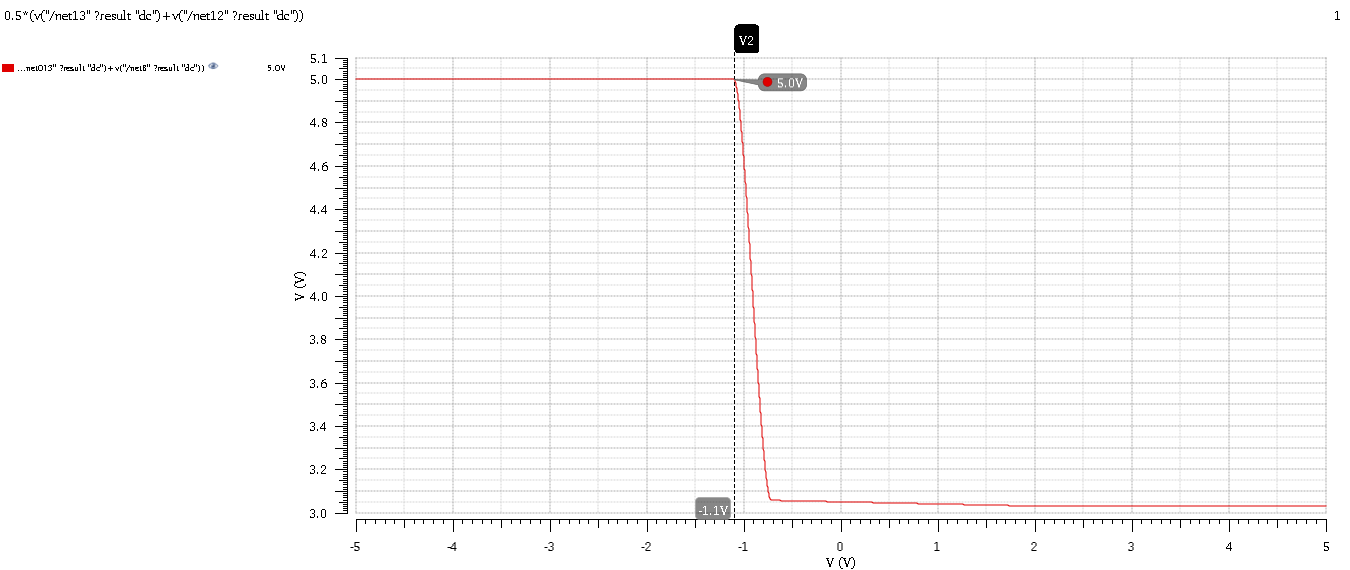
\includegraphics[scale=0.40]{./images/sim3_bigrange.PNG}
	\caption{CM Input Voltage Sweep from $-5$\si{\volt} to $5$\si{\volt}}
	\label{fig:sim3_bigrange}
\end{figure}

\FloatBarrier

The transistors are observed to enter cutoff around $V_{in,cm}=-1.1$\si{\volt}.
The linear region should also have both transistors in saturation since dropping the gate voltage from saturation should not cause them to enter triode.
It is not clear that the transistor enters triode since the large-signal common-mode voltages hover about the midpoint of the saturation region's output voltage as the input voltage becomes increased. \\

\FloatBarrier

\begin{table}[h!]
	\centering
	\caption{Conditions for All Transistors to be in Saturation}
	\label{tab:sim3_sat}
	\csvautotabular{./tables/sim3_sat.csv}
\end{table}

\FloatBarrier
{\footnotesize Common-mode output voltage is acquired by taking the large-signal common-mode output voltage in the simulation and subtracting the midpoint of the saturation region's output voltage since the transistors are biased at this point anyway.}
\FloatBarrier

The simulation result for the common-mode gain is tabulated in table (\ref{tab:sim3_gain}).
The simulation result and theoretical calculation are essentially the same.

\FloatBarrier

\begin{table}[h!]
	\centering
	\caption{Common-Mode Gain Results from Simulation}
	\label{tab:sim3_gain}
	\csvautotabular{./tables/sim3_gain.csv}
\end{table}

\FloatBarrier
